% !TEX root = 0_main.tex
\chapter{Garbled Processor}
\section{Private Function Evaluation}
Two-party Private Function SFE (PF-SFE) allows secure computation of a function $f_{Alice}(\cdot)$ held by one party (Alice) operating on another party's data $x_{Bob}$ (Bob) while both the data and the function are kept private.
This is in contrast to the usual setting of SFE where the function is known by both parties.
PF-SFE is especially useful when the function is proprietary or classified.

It is well known that PF-SFE can be reduced to regular SFE by securely evaluating a Universal Circuit (UC) \cite{sander1999non}.
UC is a circuit capable of simulating any circuit (function) $f(\cdot)$ given the description of $f(\cdot)$ as input \cite{valiant1976universal,kolesnikov2008practical}.
More formally:
$$UC(f_{Alice}(\cdot),x_{Bob}) = f_{Alice}(x_{Bob}).$$
Secure evaluation of UC completely hides the functionality of $f(\cdot)$, including its topology.
Subsequent works have shown how to allow PF-SFE while avoiding the overhead of UCs \cite{katz2011constant, mohassel2013hide}.

A UC is similar to a Universal Turing Machine (UTM) \cite{turing1936computable,herken1995universal} that receives a Turing machine description $f_{Alice}(\cdot)$ and applies it to the input data ($x_{Bob}$) on its tape \cite{davis2001engines}.
One party provides the machine description and the other one provides the initial data.
The output $f_{Alice}(x_{Bob})$ resides on the tape after the operation is completed.
A general purpose processor is a special realization of a UTM.
It receives a list of \emph{instructions} $f_{Alice}(\cdot)$ and applies them to the input data $x_{Bob}$ in memory.

\subsection{Arithmetic Logic Unit}
The core of conventional processors is the Arithmetic Logic Unit (ALU) which receives two \emph{operands} and an \emph{opcode} indicating the desired operation.
ALU supports an operation set consisting of operations like addition, multiplication, XOR, etc.
The ALU circuit consists of multiple sub-circuits for these operations and a MUX which selects one of their outputs.
Secure evaluation of an ALU, where the opcode comes from one party and operands come from the other party, keeps the operations private.
Thus, ALU can be thought of as an emulator of a simple UC in which the input function $f_{Alice}(\cdot)$ is limited to a single operation.

One can combine a number of ALUs to make a more comprehensive UC that can support functions consisting of multiple operations.
Unfortunately, this approach is not practical as the complexity of the circuit grows linearly with the number of operations.
On the other hand, in conventional processors, ALUs are combined with arrays of FFs, a.k.a., \emph{registers}, in order to store the intermediate values for supporting functions with arbitrarily large number of operations.
Since none of the earlier implementations of GC explicitly supported memory elements such as FFs, the ways to connect the feedback loop around the ALU were rather limited.
However, an explicit sequential description supported by SkipGate allows us to leverage conventional processor architectures.
Therefore, the SkipGate methodology not only provides a powerful method for generating compact circuits with a low overhead for SFE, but also paves the way for systematically building scalable sequential circuits that can be used for PF-SFE.

The idea of using an ALU or a \emph{universal next-instruction circuit} in the GC protocol can also be found in \cite{liu2014automating}.
The objective of that paper was improving efficiency of SFE where the function is known by both parties, unlike PF-SFE where the function is private.
Nonetheless, instead of ALU they eventually decided to use an \emph{instruction-specific circuit} which leaks information about the function but results in less effort for non-private function evaluation.

\subsection{Memory}
The processor accesses the memory while executing an instruction to read the instruction and data and write the data back.
If the memory is securely evaluated along with the processor, the access patterns must be also oblivious to both parties.
On the other hand, if the memory is not evaluated securely, the access patterns could be revealed that in turn could reveal information about the function to Bob and about the data to Alice.
For example, the instruction read pattern discloses the branching decisions in the function which may leak information about the data.
Because of SkipGate sequential methodology, the memory can be easily implemented using MUX and arrays of FFs.
Thus, it can be included in the processor circuit to be evaluated securely using the GC protocol.
However, inclusion of MUXs and FFs increases the operation time and communication linearly with respect to the memory size.

One alternative approach for hiding memory access patterns is the use of Oblivious Random-Access Machine (ORAM) protocols \cite{goldreich1996software} which allows oblivious load/store operations with amortized polylogarithmic overhead \cite{gordon2012secure,liu2014automating,lu2013garble,gentry2014garbled}.
For the sake of simplicity, we do not use ORAM in this work.
However, one can simply connect our implementation of PF-SFE to an ORAM to benefit from its lower amortized complexity.
As another alternate, \cite{zahur2013circuit} showed that algorithms can sometimes be rewritten to use data structures such as stacks, queues, or associative maps for which they give compact circuit constructions of poly-logarithmic size.

\section{Garbled MIPS}
\subsection{Secure Processor}
We assume Alice provides the private function $f_{Alice}(\cdot)$ and Bob provides private data~$x_{Bob}$.
At the end of the operation, only Bob learns the output $f_{Alice}(x_{Bob})$.
Note that we are not considering the case where both parties learn the output as that would allow Alice to learn Bob's private data with an identity function ($f\equiv I$).
The protocol is as follows:

\begin{enumerate}
\item
  Alice and Bob agree on an instruction set architecture (ISA), its implementation (i.e., the processor circuit), the maximum number of sequential cycles, and the configuration of data $x_{Bob}$ in the memory.
\item
  Alice compiles the function $f_{Alice}(\cdot)$ according to the ISA.
  Her input is the compiled binary of the function.
\item
  Bob prepares his input based on the agreed configuration to initialize the processor memory.
\item
  Using any secure GC framework, Alice garbles the processor circuit for the maximum number of sequential cycles and Bob, after receiving his inputs with OT, evaluates the garbled processor circuit for the same number of cycles.

\item
  Alice reveals the output types such that Bob learns the value of the output $f_{Alice}(x_{Bob})$ stored in memory.
  This needs to be done only for agreed memory locations containing the outputs such that Bob does not learn intermediate values in the memory.
\end{enumerate}

Because of secure evaluation using the GC protocol in Step 4, no information about values in the circuit will be leaked except the output.
Without knowing internal values in the processor circuit, none of the parties can distinguish instructions or memory access patterns.
In the following, we demonstrate an implementation of a processor supporting the MIPS (Microprocessor without Interlocked Pipeline Stages) ISA, as an example of a garbled processor for securely evaluating private functions.

\subsection{MIPS}
MIPS is a text-book Reduced Instruction Set Computing (RISC) ISA \cite{kane1992mips}.
The RISC ISA consists of a small set of simplified assembly instructions in contrast to Complex Instruction Set Computing (CISC) (e.g., x86 ISA) which includes more complex multi-step instructions \cite{hennessy2012computer}.
We choose a RISC ISA processor instead of CISC for the following main reasons: (i) lower number of non-XOR gates, (ii) simple and straightforward implementation, and (iii) availability and diversity of open-source implementations.
Moreover, we choose a single-cycle MIPS architecture (i.e., one instruction per sequential cycle).
Other architectures (i.e, multi-cycle and pipelined) increase the performance of the processor by parallelization.
However, the GC protocol does not benefit from such low level parallelization.
The only important factor for GC is the total number of non-XORs which is smaller in the single-cycle MIPS.
We follow the Harvard Architecture which has distinct instruction memory (IM) and data memory (DM) in order to separate the parties' inputs.
IM is a Read-Only Memory (ROM) that stores Alice's instructions.
DM is a Random Access Memory (RAM) that is initialized with Bob's input.
The parties' inputs are connected to the initial signal inputs of FFs in the memories.
Bob's outputs are connected to the outputs of FFs in the specified address of DM.
The output address in DM is part of the agreed memory configuration.

\begin{figure}[ht]
\centering
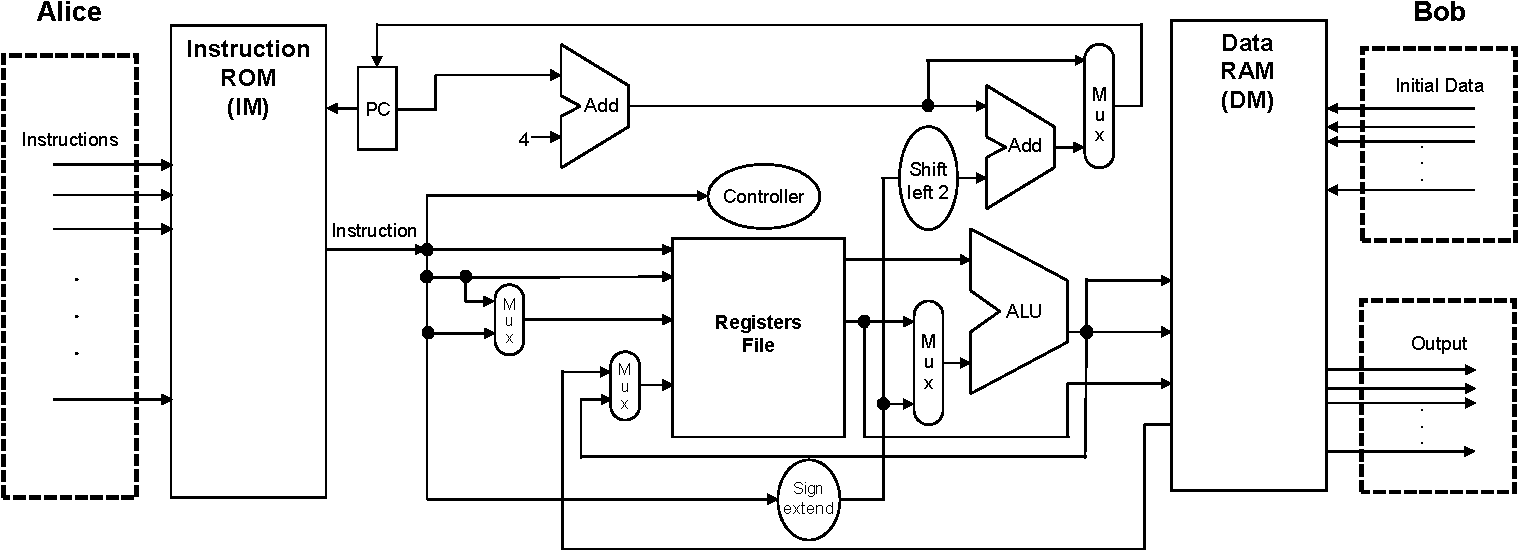
\includegraphics[width=0.95\textwidth]{mips-complex-crop.pdf}
\caption{Lite MIPS architecture.
  Alice's and Bob's inputs and the output are shown.}\label{figure:mips}
\end{figure}

\fig{figure:mips} shows the overall architecture of our 32-bit MIPS processor.
It is based on the Plasma project in opencores \cite{rhoads2006plasma}.
We modified the circuit such that the instruction ROM (IM) and the data RAM (DM) are separated.
The original Plasma processor supports all the MIPS~I ISA except unaligned memory access.
In our implementation, we also omit division instructions because of their large overhead.
Any arbitrary C/C++ function can be easily compiled to MIPS~I assembly code using a cross-platform compiler e.g., GNU gcc.

In 32-bit MIPS, the program counter (\emph{PC}) is a 32-bit register (array of FFs) that points to the instruction being executed at the current cycle.
The instruction is fetched from IM based on the current PC value.
The \emph{controller} unit is responsible for setting signals to perform the instruction.
In 32-bit MIPS, the \emph{register file} consists of 32 registers of 32-bit each.
In each cycle, at most two registers can be read and at most one register can be written back.
ALU receives the read register(s) or a sign extended \emph{immediate} as operands.
ALU also receives an opcode from the controller unit.
The output of ALU will be either written back to the register file or fed to DM as an address for load/store.
The loaded data from DM is written back to the register file.
In each cycle, PC is incremented by 4 to point to the next instruction in IM or is changed according to a branch or jump instruction.

\section{Garbled Processor}
The idea of garbling a processor was first introduced in \cite{songhori2015tinygarble} as a solution for hiding the function in PF-SFE. Besides enabling PF-SFE, another advantage of a garbled processor is usability for non-expert users since it can be programmed using high-level languages, whereas other frameworks for the GC protocol require tedious Boolean circuit construction. However, garbling and evaluating the entire processor incurs a tremendous cost compared to SFE solutions due to stronger privacy requirements in PF-SFE.

\paragraph*{Adversary Model} We assume an honest-but-curious (i.e., semi-honest or passive) adversary which is sufficient for most practical scenarios to enable efficient protocols. This establishes the first step towards protocols with stronger security guarantees against malicious or covert adversaries.

In this work, we propose GarbledCPU as a hardware-only garbled processor framework for secure computation that provides scalable support for generalized SFE with a relaxed privacy setting but improved performance, besides the more security-demanding PF-SFE, as well as a flavor in-between. To avoid information leakage about the function (i.e., PF-SFE), we use GarbledCPU with its full Instruction Set (IS), which incurs a large overhead due to garbling and evaluating of the entire IS. We can also compile the function using only a subset of the IS: restricted IS (i.e., semi-private function). A third alternative is public function mode in which the function is compiled using only an application-specific subset of the IS that is required for executing the function. In the following, we discuss these modes of function evaluation and the trade-off between privacy and performance further.

\fig{fig:oview} shows the overview of GarbledCPU for 2-party computation between Alice (garbler) and Bob (evaluator). Alice generates the garbled instructions and tables by garbling the processor circuit for the selected IS mode and sends them to Bob. He also receives his garbled input data through OT from Alice without revealing his input to her. Bob evaluates GarbledCPU and produces the garbled output. Eventually, Alice reveals the output map to Bob and he ``ungarbles'' and learns the output data.

\begin{figure}[ht]
\centering
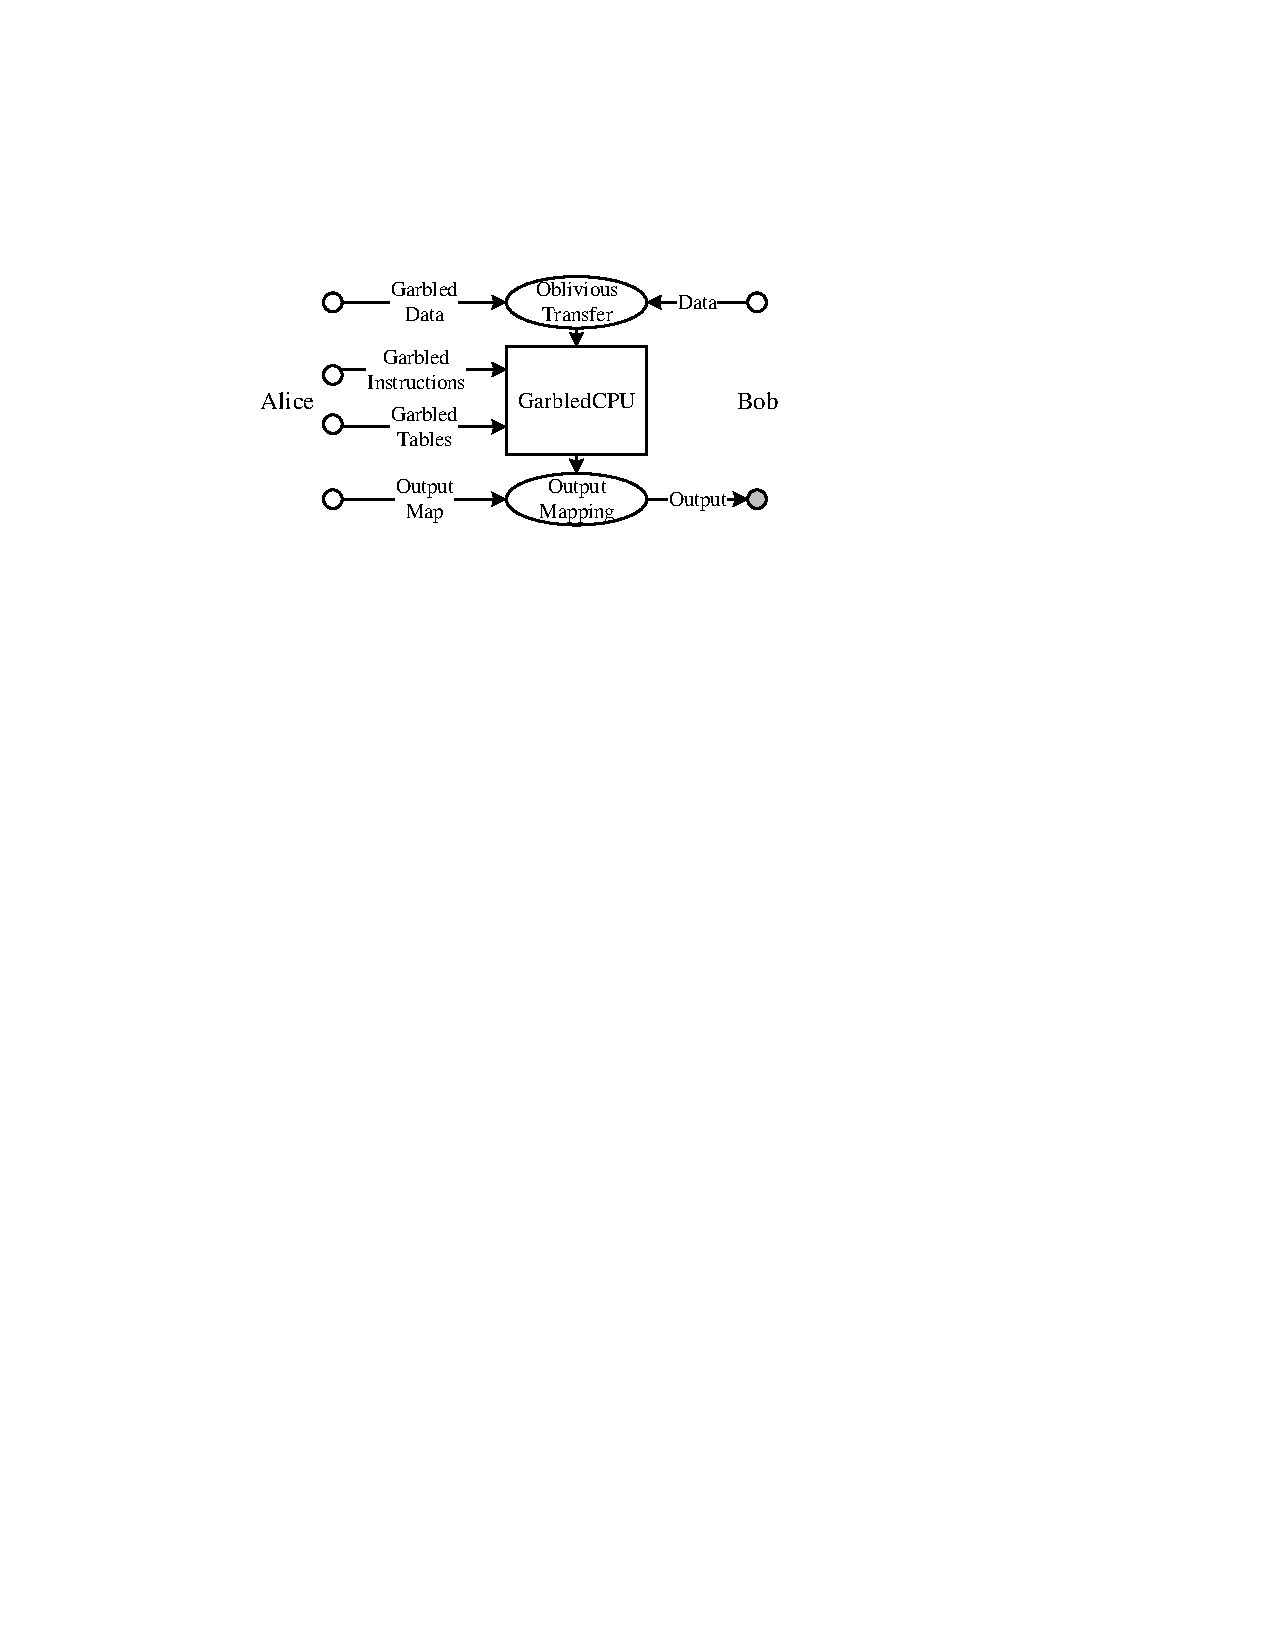
\includegraphics[width=\textwidth]{overview-crop.pdf}
\caption{Overview of GarbledCPU.} \label{fig:oview}
\end{figure}

\subsection{Garbled Processor for Public Functions}
Using a general-purpose processor with its entire IS in SFE results in garbling a large processor which is very costly and unnecessary since both parties know the function instructions being executed but not their results.
Hence, garbling a limited application-specific IS for executing each instruction is sufficient to achieve privacy. In \sect{sect:synres} we show three examples of GarbledCPU with application-specific IS. To further reduce the IS, assuming for example, a function that consists of \numprint{10} instructions, we could theoretically generate $2^{10} -1$ netlists (netlists of IS with different combinations of the 10 instructions, excluding the netlist with zero instructions). At run-time, one of these netlists is plugged in (garbled and evaluated) at each instruction step depending on the expected instructions. However, to make it more reasonable (generate fewer netlists), for functions with control flow independent of private data, we know in advance which instruction will be executed at each step. Thus, we need only the netlist of the processor implementing IS with that specific instruction, restricting the required netlists in this case to \numprint{10}. For functions with control flow dependent on private data, a simple static analysis can be used to specify the combination of possible instructions at each step, and hence the required IS netlist as proposed in \cite{wang2015secure}.

\subsection{Garbled Processor for Semi-Private Functions}
The main cost for garbling a processor with its entire IS results from garbling circuits for expensive instructions like multiplication and division. Most compilers are able to avoid these costly instructions and replace them with cheaper loops of shifts, addition, and subtraction instructions. This would eliminate the need for the Mult/Div unit in the processor and reduce the cost of garbling per instruction on one hand. However on the other hand, one expensive instruction will be replaced with multiple cheap instructions, thus increasing the total number of instructions. For example, multiplying two 32-bit numbers with the MULT instruction in MIPS requires \numprint{15} cycles and a circuit of \numprint{13257} non-XOR gates\footnote{XOR gates are evaluated freely in GC according to the free-XOR optimization of \cite{kolesnikov2008improved}.}, while it requires at least \numprint{31} cycles and a circuit of \numprint{9,676} non-XOR gates when using a conditional loop over an ADD instruction. We call this mode ``semi-private'' since it only reveals partial information about instructions used in the program (that the program does not use division/multiplication) and increases the probability of guessing an instruction by reducing the subset of possible instructions (restricted IS).

\subsection{Garbled Processor for Private Functions}
In the standard 2-party PF-SFE, Alice provides the function $f_{Alice}(\cdot)$ and Bob provides the input data $x_{Bob}$ and the output is $f_{Alice}(x_{Bob})$. In this work, GarbledCPU receives a list of \emph{instructions} as $f_{Alice}(\cdot)$ and applies them to the input data $x_{Bob}$ in memory and the output will be written back to the memory. To avoid information leakage about the private function, we use a general-purpose processor with its entire IS (full IS).

\section{GarbledCPU Implementation}
We present our garbled processor in \sect{ssect:mips}, a high performance hardware architecture for GC to evaluate GarbledCPU in \sect{ssect:hwimp}, and implementation challenges in \sect{ssect:challenges}.

\subsection{MIPS}
To implement GarbledCPU, we use the MIPS architecture from the Plasma project in Opencores \cite{rhoads2006plasma}. We chose the single-cycle implementation of the 32-bit MIPS I instruction set which is based on the Reduced Instruction Set Computing (RISC), making its Boolean representation among the simplest of modern processors. Note that the gates should be garbled/evaluated one after another in the GC protocol, and it is challenging to benefit from physical level parallelism that exists inherently in hardware. Thus, using a multi-cycle, pipelined, or a more sophisticated architecture not only complicates the implementation, but also counter-intuitively, increases the overall cost of garbling for the same functionality. The time required for garbling a circuit depends only on the total number of gates and not the critical path. In \sect{sect:synres} we present the garbling cost for MIPS with various memory sizes.

\subsection{Our Hardware Architecture}\label{ssect:hwimp}
To the best of our knowledge, the fastest implementation of GC is JustGarble \cite{bellare2013efficient}. JustGarble is a software GC realization using fixed-key AES garbling which benefits from the AES-NI instruction set in modern Intel processors. Its performance reaches about $20$ clock cycles per gate for GC evaluation. Prior to JustGarble, J\"arvinen et al. introduced two hardware realizations for the GC protocol in \cite{jarvinen2010garbled}. However, their performance is much slower than JustGarble because JustGarble utilizes a more efficient fixed-key AES for garbling instead of an expensive hash function. Thus, it is possible that a hardware implementation leveraging the latest GC optimizations including fixed-key AES garbling would outperform JustGarble. Furthermore, a processor is essentially a sequential circuit and its evaluation requires sequential GC which none of these works supports.

Our GC evaluator is based on the most recent optimizations listed in \sect{ssect:gc}. Its architecture is shown in \fig{fig:evaluator} and consists of:
(1) Simple Circuit Description (SCD) memory: read-only memory that stores the information about gates in the MIPS circuit in SCD format \cite{bellare2013efficient, songhori2015tinygarble}.
(2) GC Label memory: read-write random-access memory that stores GC ciphertext labels of all wires in the corresponding MIPS circuit.
(3) Garbled Tables (GT) memory: read-write random-access memory that stores the ciphertext garbled tables of each non-XOR gate in the MIPS circuit that are generated by Alice (garbler).
(4) Sequential Handler: controller that supports evaluation of the sequential circuits with the GC protocol.
(5) Evaluator Engine: main functionality of GC evaluation according to Yao's GC protocol and its most recent optimizations \cite{kolesnikov2008improved, bellare2013efficient, zahur2015two,songhori2015tinygarble}.

As shown in \fig{fig:evaluator}, Bob's input labels in the Label memory are initialized by the OT protocol with Alice. The rest of the labels in the Labels memory and the Garbled Tables memory are received in clear-text from Alice.


\begin{figure}
\centering
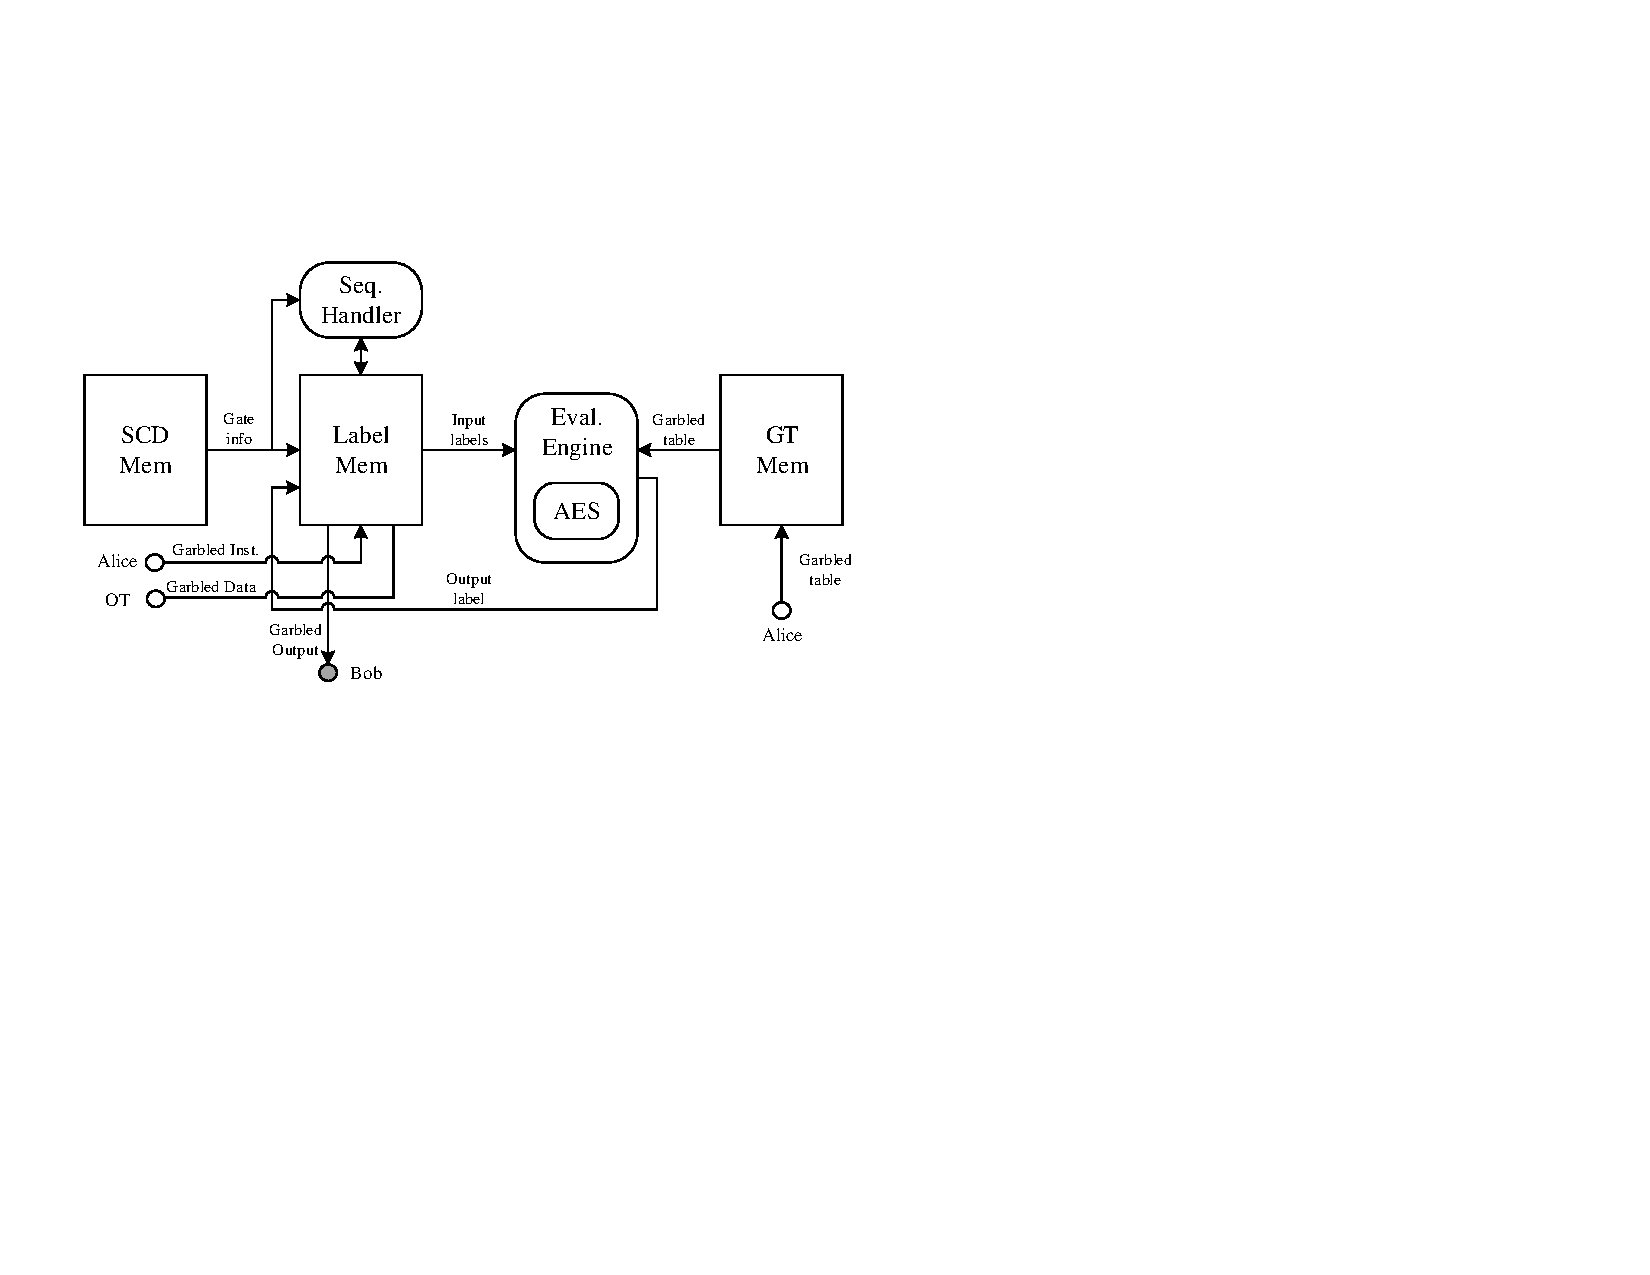
\includegraphics[width=\textwidth]{Evaluator-crop.pdf}
\caption{Our GC Evaluator Architecture.}
\label{fig:evaluator}
\end{figure}

\paragraph*{Pipelined Evaluator Engine and Gate Dependency}
To maximize the performance of the GC evaluator, we use a 20-stage pipelined AES implementation \cite{hsing2013tiny} inside our Evaluator Engine module. It increases the throughput of the module by increasing the maximum operating clock frequency of the engine. We also add one stage for the rest of the GC evaluation functionality.
%
Due to the free-XOR technique \cite{kolesnikov2008improved}, evaluating an XOR gate requires only XOR-ing the input labels while evaluating a non-XOR gate requires two AES encryptions (due to half-gates technique presented in \sect{ssect:gc}, and was one encryption before). Therefore, evaluation of an XOR gate can be done in only one stage of the AES pipeline. Different timing for XOR and non-XOR gates introduces a challenge for handling dependencies of gates' inputs and output. A gate cannot enter the evaluation pipeline if its inputs are another gate's output which is not yet evaluated. This results in pipeline stalls which degrade the overall performance. To mitigate this, we push XOR gates to the latest empty stage of the pipeline such that the subsequent dependent gates can enter the pipeline as soon as possible.

\subsection{Hardware Prototype Challenges}\label{ssect:challenges}
We only use on-chip memory for our proof-of-concept in this work. However, this prototype can be extended to support interfacing with off-chip memory which would store garbled tables and labels of larger garbled processor circuits and functions. It can also interface with another FPGA emulator of the garbler which generates the garbled tables and labels and streams them to our evaluator. A wide range of scenarios are now feasible owing to our current hardware platform and state-of-the-art optimized GC evaluator.
%
Such extensions would incur additional area and performance overheads, but would allow upscaling of our implementation to support garbled processor circuits and benchmarks in the Gigabytes range. We emphasize that we provide in this work a proof-of-concept prototype to motivate further research in this direction to bring garbled processors some steps closer to the realm of feasible practical implementations.

\section{ARM2GC}
The ARM2GC framework allows users to write two-party SFE program in C/C++ (or any language that can be compiled to ARM binary code).
\fig{fig:frwk_overview} shows the overview of the framework.
The SFE program is compiled using an ARM cross-compiler, e.g., gcc-arm-linux-gnueabi.
The compiled binary code and the synthesized ARM processor circuit are fed to the SkipGate algorithm as a public input and netlist respectively.

\begin{figure}[ht]
\centering
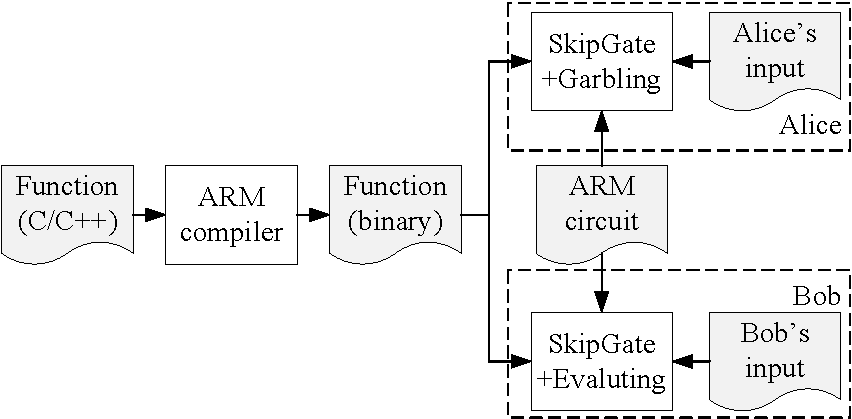
\includegraphics[width=0.45\textwidth]{frwk_overview-crop.pdf}
\caption{Overview of the ARM2GC framework.}\label{fig:frwk_overview}
\end{figure}

The ARM2GC framework supports the following API:
\begin{lstlisting}[language=C,basicstyle=\ttfamily,keywordstyle=\color{blue}\ttfamily,stringstyle=\color{red}\ttfamily,commentstyle=\color{CommentColor}\ttfamily]
void gc_main(
  const int *a,// Alice's input
  const int *b,// Bob's input
  int *c) {// output array
  // The user's code goes here.
}
\end{lstlisting}

The entry function, \texttt{gc\_main}, receives three arguments: pointers to Alice's input, Bob's input, and the output.
The framework has five separate memory elements (consisting of flip-flops and MUXs) to store: Alice's inputs, Bob's input, output, stack, and instruction.
The flip-flops in the instruction memory are initialized with the compiled binary code that is known to both parties (the public input $p$).
The flip-flops in Alice's and Bob's memories are initialized with the labels corresponding to their private inputs $a$ and $b$ respectively.
The other flip-flops in stack, output, pipeline registers, and register files are initialized to zero.
The netlist is garbled/evaluated for a pre-specified number of cycles.

\subsection{How SkipGate Helps}
Implementation of ARM processor results in a complex and large netlist ($\approx 5$ times larger than MIPS).
Thus, using ARM instead of MIPS in the previous garbled processor approaches~\cite{wang2015secure, songhori2016garbledcpu} would incur even higher cost.
However, majority of the components of the ARM processor remain idle during  execution of an instruction.
SkipGate utilizes this to minimize the cost of garbling the ARM processor.
Since the instruction memory is initialized with public values, if the program counter (the address of the next instruction) is public, the next instruction becomes public.
As a result, the control path also becomes public and SkipGate can detect the idle components to mark them for skipping.
Moreover due to SkipGate, the gates of the active components that are only transporting data between memory, register file, and ALU act as wires and do not incur any cost.
Therefore, the main garbling cost is paid for the actual computation on the secret values inside the ALU.
As explained in the previous section, SkipGate performs these optimizations at the gate-level, in contrast to instruction-level of~\cite{wang2015secure, songhori2016garbledcpu}.

\subsection{ARM as a Garbled Processor}\label{ssect:arm}
In this work, we choose ARM as our garbled processor which is a more ubiquitous and sophisticated processor compared to MIPS~\cite{songhori2015tinygarble, wang2015secure, songhori2016garbledcpu}.
ARM has two main advantages:
(1) Pervasiveness: the compilers and tool-sets of ARM are under constant scrutiny, updating, and probably, more optimized as a result.
(2) Conditional Execution: Designed to improve performance and code density, conditional execution in ARM allows each instruction to be executed only if a specific condition is satisfied~\cite{sloss2004arm}.

ARM compiler tends to replace conditional branches with conditional instructions to make the flow of the program predictable, and thus, lower the cost of branch mis-prediction.
Similarly in garbled processor, the main design effort is to make sure that the flow of the program is predictable so that the next instruction is public.
Replacing conditional branches with conditional instructions in garbled ARM generates a code with a predictable flow.
\fig{fig:conditional_exec} shows an example function compiled into assembly with and without the conditional execution.
Moreover, we modify the ARM controller such that a conditional instruction always takes the same number of cycles regardless of its condition.
This is because when the condition is secret, mismatch in the number of cycles of the instructions makes the program flow dependent on a secret value.

\begin{figure}[ht]
    \centering
    \begin{subfigure}{0.40\textwidth}
        \centering
        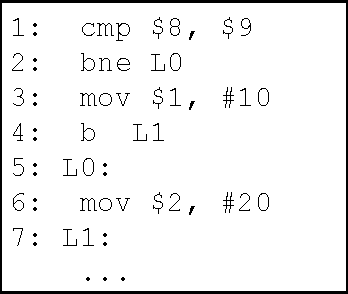
\includegraphics[width=\textwidth]{conditional_exec_wo-crop.pdf}
        \caption{Without Conditional Execution}
    \end{subfigure}
    ~
    \begin{subfigure}{0.40\textwidth}
        \centering
        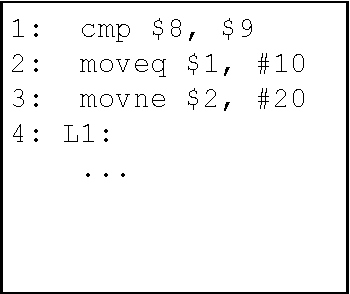
\includegraphics[width=\textwidth]{conditional_exec_w-crop.pdf}
        \caption{With Conditional Execution}
    \end{subfigure}
    \caption{An example code showing how conditional execution in ARM can reduce the code size and make the program flow predictable.}\label{fig:conditional_exec}
\end{figure}

We modify and remove a few features from the ARM processor like interrupts, co-processors, and performance-related components including cache and pipeline.
The last group does not bring any performance advantages in the GC protocol, as the circuit is garbled/evaluated gate by gate (serially).
Note that unlike in hardware, the performance of GC does not increase by parallelizing gates in the circuit.
In the GC protocol, the total number of non-XOR gates is the only factor affecting the performance, not the circuit's topology.
